\chapter{Project Overview}

\section{Introduction}

Our group is seeking to develop a reinforcement learning agent to support portfolio 
management and optimization. Utilizing both empirical stock pricing data along with 
alternative data, we look to create a more well-informed portfolio optimization tool. 

Our primary motivations for pursuing a reinforcement learning-based approach are as 
follows:

\begin{enumerate}
    \item Reinforcement learning lends itself well to learning/opening in an online environment. The agent can interact with its environment, providing real-time feedback/ responsiveness to allow for better results.
    \item Our approach involves incorporating alternative data to support the agent’s decision making process. Encoding this alt-data into the states matrix of the agent allows for the agent to make better decisions when it comes to adjusting portfolio weights.
    \item Given that a reinforcement learning agent’s decisions are modeled by a Markov Decision Process, we can easily provide different reward functions to account for a variety of investor preferences or restrictions.
\end{enumerate}



\section{Dataset Creation}

Creating a combined dataset encompassing a textual corpus sufficient for us to build 
a robust reinforcement learning agent will require pulling data from a wide variety 
of sources. We aim to use two primary types of data: stock and news data.

\subsection{Stock Data}

We retrieve data from Wharton Research Data Services 
(WRDS). WRDS is a pre-eminent source of financial data that we have experience 
utilizing in the Computational Finance program’s other courses that has expansive 
data on stocks. Specifically, we want to utilize data from the Center for Research in 
Security Prices (CRSP), which has security price, return, and volume data for stocks listed in the 
NYSE, AMEX and NASDAQ exchanges. We created a our trading universe with the S$\&$P 100 stocks.

\subsection{News Data}

An important direction of our research is to explore how the performance 
of reinforcement learning trading agents are influenced by news data.
We believe that news data will impart an external understanding of how 
well a given stock is performing at a given time and its exposure market or sector risks. 
This could provide our agent a better view of the trading environment, which 
can help it make better decisions to maximize the reward. 

The dataset we use in this project is Daily Financial News for 6000+ Stocks that was downloaded via kaggle \cite{financial_news}.
This dataset contains scraped headline data for over 6000 stocks listed on the NYSE exchange from 2009-2020. 
There are two main files within this dataset that we use. The first is \texttt{raw\_analyst\_ratings.csv}, which only contains scraped data from a prominent finacial news publisher Benzinga.
The other file \texttt{raw\_partner\_headlines.csv} contains scraped headline data from other smaller publishers that partner with Benzinga. Each row of the file contains a headline, the base article URL, the date and time of publication, and the stock ticker symbol.
The \texttt{raw\_analyst\_ratings.csv} file does not contain publisher information, as it is already implied that Benzinga is the publisher. Meanwhile, the table in \texttt{raw\_partner\_headlines.csv} has a column indicating the publisher of each article. 
We concatenate the headline data from each file into one unified dataset that contains all headlines for each stock in our universe.


\subsubsection{SEC Filings}

To enrich our dataset, we utilize SEC filings data for each of the S$\&$P100 companies. 
These filings contain essential information regarding a company's financial 
performance, governance, and compliance that could enhance our measure of 
company outlook. Specifically we aim to use data from 10-K and 10-Q filings. 
10-K’s are an annual report on a company’s performance, and include information. 
They are divided into items that show a company’s financial statements, 
stock projections, and pertinent information for shareholders in sections that 
are denoted as items. 

For the 10-k reports for For our project, the textual data that is most likely to 
capture a company’s sentiment is Item 1A, Risk Factors. This item is a company 
issued statement on the risk factors that could affect the operations of the 
business for the next fiscal year. We will extract this data from 10-K statements 
for every company in our trading universe to create sentiment indicators for our 
RL agent to use. 

\subsection{Sentiment Analysis}

Using the news sources and SEC filings data described above, we wish to 
generate embeddings from which we can extract sentiment related features 
to provide to our reinforcement learning agent. Our approach, which is to utilize the pre-trained 
FinBERT model, fine-tuned to recognize the sentiment of financial text to 
create embeddings for us \cite{finbert}. 

\subsubsection{FinBERT Sentiment Scores}

Over the full trading period (2010-2015), we will feed all of the headlines to pre-trained FinBERT. 
The model then will preprocess the text and generate probabilities of the content 
being positive, negative, or neutral. From there, we can assign each headline a 
numerical score based on its maximum probability class. The numerical map could 
look something like the following:  {positive: 1, neutral: 0, negative: -1} 
Over each day (our trading period), we can take some aggregate of these class labels for 
each stock and feed these class labels to our agent’s states matrix; at each 
time step, this value will be appended to the row corresponding to the stocks’ 
price data. (The state matrix will be defined in greater detail in the Algorithmic 
and Analytical Challenges section.) We ran experiments using different aggregation functions
aggregate function which include taking the mean of the sentiment mappings for each day, and designing a custom function to extract value heuristically. 
The function that we created is:
\[\texttt{Value}_{\texttt{Embedding}} = \tanh\Biggl( \frac{\frac{\texttt{positive sentiment probability}}{\texttt{negative sentiment probability}}}{\texttt{neutral sentiment probability}} \Biggr)\]
This approach combines the “log likelihood” (ratio of probabilities of positive and 
negative sentiment) along with a penalty for high neutral sentiment (a measure of 
uncertainty), using the tanh for normalization. This approach would allow us to 
adequately detect strong positive/negative sentiment. 

We will test the exact same preprocessing pipeline on the SEC 10-K and 10-Q filings 
for each company in our universe and integrate them into our states matrix. An issue that incorporates SEC filings is that they are recorded on a 
relatively infrequent basis compared to news and price data. Thus, we have also experimented with functions that model the decay of the sentiment.
The experiment that we run is using exponential decay, that is we assume that the weight of our news sentiment signal decays by some constant rate $\lambda$ over time. Formally,

$$
\frac{dN}{dt} = -\lambda N
$$

Where $N$ represents the company's sentiment score for the day, $t$ represents time (in days), and $\lambda$ is a positive constant representing the daily rate of decay. We test $\lambda = 0.1, 0.5, 0.9$ in our models to see what performs optimally. Note that we test such a wide range of $\lambda$ values because we are unsure of how fast the trading signal from news sentiment scores decays.
 
We also compare this strategy against a baseline assumption that there is no information carried forward for headline data. That means sentiment embeddings for each company will only be updated on dates where a
new filing was reported. On non-reporting dates, the embeddings will be filled 
forward from the last filing date. 


\section{Algorithmic and Analytical Challenge}

Our primary model technique is deep reinforcement learning, which is a 
branch of machine learning that operates in a game-theoretic-like system. 
Formally, a reinforcement learning problem is an instance of a Markov 
Decision Process, which is a 4-tuple $(S, A, T, R)$: $S$ the state space 
(matrix of selected historical stock price and news data available to 
our model at a given time; see Methodology section), $A$ the action space 
(portfolio weights produced by our model, under appropriate constraints), 
$T$ the transition function (how the state changes over time, modeled by our dataset), 
and $R$ (the reward function). The goal is to find a policy (function from $S \to A$) 
that maximizes future expected rewards. Most reinforcement learning research is 
spent on providing good information in $S$ to the model, defining a good reward 
function $R$, and deciding on a deep learning model training system to optimize rewards.

\subsection{Existing Literature}

Much of the literature applying RL to portfolio optimization has arisen in the 
last few years. Some relevant papers are:

\begin{itemize}

\item \cite{drl_mvo} Deep Reinforcement Learning Comparison with Mean-Variance Optimization: 
Using a lookback of recent past returns and a few market indicators 
(including 20-day volatility and the VIX), this paper implements a simple 
algorithm for portfolio weight selection to maximize the Differential Sharpe Ratio, 
a (local stepwise) reward function which approximates (global) Sharpe Ratio of the 
final strategy. They compare their model with the standard mean-variance 
optimization across several metrics.

\item \cite{drl_modern_portfolio_theory} DRL for Stock Portfolio Optimization Connected with Modern 
Portfolio Theory: This paper applies reinforcement learning methods to 
tensors of technical indicators and covariance matrices between stocks. 
After tensor feature extraction using 3D convolutions and tensor decompositions, 
the DDPG method is used to train the neural network policy, and the algorithm 
is backtested and compared against related methods.
 
\item \cite{rl_augmented_states} RL-Based Portfolio Management with Augmented Asset Movement Prediction 
States: The authors propose a method to augment the state space S of historical 
price data with embeddings of internal information and alternative data. 
For all assets at all times, the authors use an LSTM to predict the price movement,
which is integrated into S. When news article data is available, different NLP methods 
are used to embed the news; this embedding is fed into an HAN to predict price 
movement, which is also integrated into S for state augmentation. The paper applies 
the DPG policy training method and compares against multiple baseline portfolios on 
multiple asset classes. It also addresses challenges due to environment uncertainty, 
sparsity, and news correlations.

\item \cite{drl_framework} A Deep Reinforcement Learning Framework for the Financial Portfolio Management Problem: 
This paper contains a deep mathematical and algorithmic discussion of how to properly incorporate 
transaction costs into an RL model. The authors also have a GitHub with implementations of their 
RL strategy compared with several others.

\item \cite{learn_to_rank} Stock Portfolio Selection Using Learning-to-Rank Algorithms with News Sentiment: 
After developing news sentiment indicators including shock and trends, this paper applies 
multiple learning-to-rank algorithms and constructs an automated trading system with strong performance.

\item \cite{maps} MAPS: Multi-agent Reinforcement Learning-based Portfolio Management System: 
This paper takes advantage of reinforcement learning with multiple agents by defining a 
reward function to penalize correlations between agents, thereby producing multiple orthogonal 
(diverse) high-performing portfolios.

\end{itemize}

\subsection{Methodology}

We will be implementing, combining, and improving on the methodologies of several of the above papers. 
Our plan is to develop an RL system that utilizes multiple time periods to achieve strong out-of-sample 
trading performance. As of this writing, we have partial implementations of papers \cite{drl_mvo}, \cite{drl_modern_portfolio_theory}, and \cite{drl_framework}.
 Our final architecture will be most similar to papers \cite{rl_augmented_states} and \cite{drl_framework}.

\subsubsection{Markov Decision Process Problem Formulation}

Paper \cite{rl_augmented_states} includes the following diagram, which is very close to our desired 
architecture:

\begin{center}
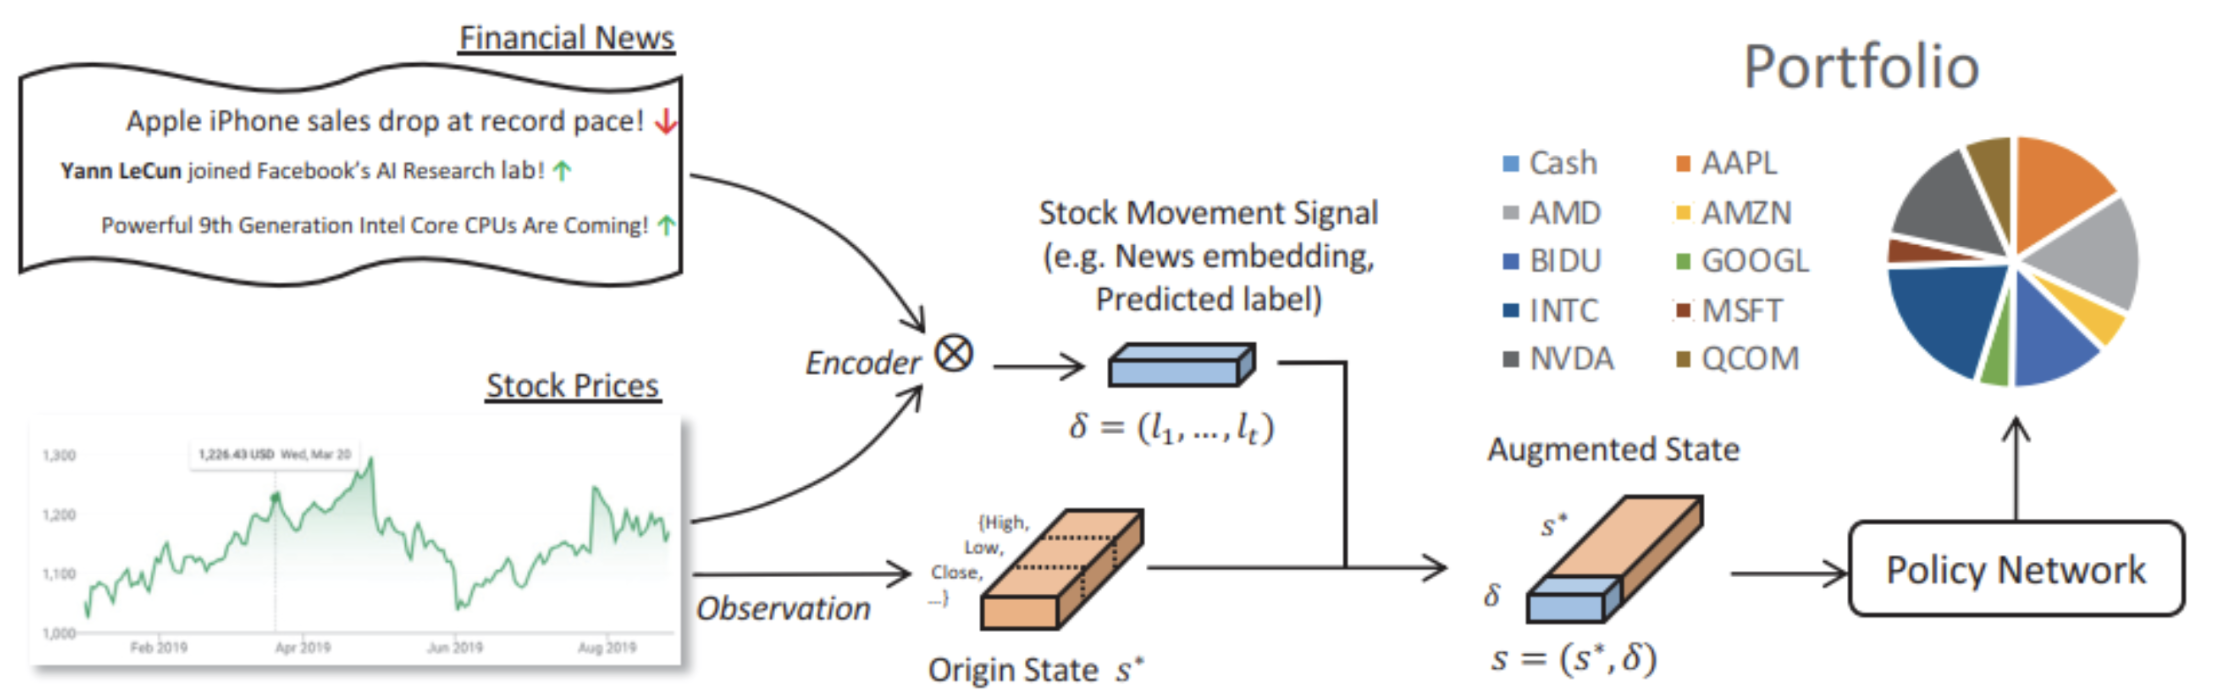
\includegraphics[width=13cm]{formulation.png}
\end{center}

An explanation of this diagram: at time t, the origin state $S^*$ is a 3D tensor of dimensions $U \times H \times C$
which contains historical price data. $U$ is the size of our universe (for example, for the S$\&$P100, $U = 100$). 
$H$ is the size of history we are providing (if we are providing 30 day history, then $H = 30$). 
$C$ is a categorical value representing the close/high/low price. This format of $S^*$ allows us to store, 
for example, the last 30 days of stock price data for all companies in the S$\&$P100, for any given day. 
In addition to this, we have news information $\delta$, obtained from financial news headlines for that day, 
processed through a pre-trained encoder. This information is added to $S^*$ to create the full state 
$S = (S^*, \delta)$

In our architecture, for $S^*$, we will experiment with the lookback period size and likely reduce it 
to a 2D array by flattening along the C index, but will otherwise keep $S^*$ largely the same. For 
$\delta$, we plan to utilize better feature extraction via sentiment scores and topic modeling; 
we also plan to use different alternative data sources, as described in the Dataset Creation section. 
In addition, we will extract what company each headline refers to, so our features can be changed 
over time independently for each company as news articles enter through our environment. The final 
state S will likely be a 2D matrix, where each row represents a different company (ticker), and along 
that row we find, concatenated, the following: (1) the past month-or-so of stock price data from $S^*$, 
and (2) numerical features extracted from recent news data pertinent to that company (as described 
in the Dataset section). (The straightforward concatenation of price data and news embeddings did not 
affect the ability of the neural network-based agent to learn.)

Regarding the reward function R, we plan to experiment with both the profit reward function used in \cite{rl_augmented_states}, 
as well as the Differential Sharpe Ratio developed in paper \cite{drl_mvo}.

In summary, our project aims to implement and replicate the approach used in \cite{rl_augmented_states}, with 
some modifications to S and R as previously described. We will conduct experiments alternative data 
sources, feature extraction methods, and reward functions (both custom and from other papers listed) 
to find a good combination that allows this approach to work well on S$\&$P100 stocks; this comprises our 
novel extension/contribution.

\subsubsection{Use of Libraries}

We will mainly be using the Gymnasium library to implement the reinforcement learning environments. 
The Stable Baselines 3 library provides several policy learning techniques that we will experiment with, 
including Proximal Policy Optimization (PPO) and Deep Deterministic Policy Gradients (DDPG). 
The papers above discuss the advantages and disadvantages of multiple reward functions and constraints, 
which we will make improvements upon and provide as options to the user, if applicable.

\subsubsection{Strategy Benchmarking}

Our final model architecture will be compared against several benchmark financial portfolio selection 
models. Among these will be the CAPM, an exponential moving average strategy, linear factor models 
such as the Fama French 3/5-factor models, and the QMJ model. We will compare our returns 
in-sample and out-of-sample plots, as well as our relative performance on portfolio statistics 
including cumulative return, Sharpe Ratio, Sortino Ratio, drawdown, etc. The experiment sections 
in the above papers provide a strong reference for our methodological comparison.

